% Provenance (never printed): old terminale S material on the transformation of
% rocks in mountain belts and subduction zones (pressure, temperature, index
% minerals and the Al2SiO5 polymorphs, foliation, contact and regional
% metamorphism). Owner (Sync 0): metamorphism, lithostatic pressure, polymorph,
% index mineral/isograd/metamorphic grade, foliation/schistosity, contact and
% regional metamorphism/aureole. Blueschist and eclogite are g11.06's, the
% geotherm g11.03's, minerals and silicates g11.07's, the rock families, marble
% and slate Book 1's (g6), pressure physics': recalled, never redefined. The
% P-T diagram: figdata/grade-12/al2sio5.py (Holdaway and Mukhopadhyay 1993,
% Table 11; geotherms from Earle 7.3).
\chapter{Metamorfe gesteenten}\label{ch:g12:metamorphic-rocks}

Een laag modder bezinkt op een zeebodem en verhardt tot schalie. Begraaf haar een paar
kilometer en pers haar samen, en ze wordt leisteen, een gesteente dat splijt in
de dunne, vlakke platen van een dak. Begraaf haar dieper en heter, en haar piepkleine
schilfers groeien uit tot glinsterende mica's, waartussen rode granaten opzwellen: een schist.
Nog dieper en heter sorteren haar mineralen zich in lichte en donkere
banden: een gneis. Onderweg smolt er niets. Dezelfde modder, met dezelfde
chemische elementen, bouwde zijn mineralen gewoon opnieuw op, passend bij de plaats waar hij
was. Andersom gelezen leggen de mineralen van een metamorf gesteente vast hoe diep
en hoe heet die plaats was, en dit hoofdstuk leert ze lezen.
% ledger: earle:foliation, earle:settings

\begin{recall}
Gesteenten vallen in drie families --- stollingsgesteenten, sedimentaire, metamorfe --- en
de gesteentekringloop maakt de ene tot de andere; marmer ontstaat uit kalksteen en
leisteen uit schalie, zonder smelten (Boek 1, jaar 6). Een mineraal is een natuurlijke
vaste stof met een bepaalde chemische samenstelling en een geordende rangschikking van
atomen; de meeste mineralen van de korst zijn silicaten
(\cref{ch:g11:minerals}). Een \omterm{def:g11:lithosphere-asthenosphere:geotherm}{geotherm} is de kromme van de temperatuur tegen de
diepte onder een plaats; dicht bij het oppervlak stijgt de temperatuur met 25 tot
\qty{30}{\celsius} per kilometer (\cref{ch:g11:lithosphere-asthenosphere}).
In een \omterm{def:g11:subduction-zones:subduction}{subductiezone} wordt \omterm{def:g11:ocean-ridges:oceanic-lithosphere}{oceanische korst} die omlaag wordt gevoerd terwijl ze koud blijft,
\omterm{def:g11:subduction-zones:eclogite}{blauwschist} en daarna \omterm{def:g11:subduction-zones:eclogite}{eclogiet} (\cref{ch:g11:subduction-zones}).
Druk is een kracht gedeeld door de oppervlakte waarop ze drukt; ze wordt gemeten in
pascal, \qty{1}{Pa} = \qty{1}{N/m^2}.
\end{recall}
% ledger: usgs:metamorphic (Book 1 row), webmineral:formulas, earle:settings, earle:controls

\section{Omgevormd in vaste toestand}

\begin{definition}[Metamorfose]\label{def:g12:metamorphic-rocks:metamorphism}
\emph{Metamorfose}\index{metamorfose} is de omvorming van de
mineralen en de \omterm{def:g11:igneous-rocks:texture}{textuur} van een gesteente, in vaste toestand, wanneer het op
een temperatuur en een druk wordt gebracht die verschillen van die waaronder het is ontstaan.
Het gesteente dat het wordt, is een metamorf gesteente.
\end{definition}
% ledger: tulane:metamorphism, earle:controls

Het gesteente waarvan \omterm{def:g12:metamorphic-rocks:metamorphism}{metamorfose} uitgaat, is zijn \omterm{def:g10:soil-formation:weathering-profile}{moedergesteente}, hetzelfde woord als
voor het gesteente onder een bodem (\cref{ch:g10:soil-formation}). \omterm{def:g12:metamorphic-rocks:metamorphism}{Metamorfose} begint bij ongeveer \qty{200}{\celsius}; daaronder horen de trage
veranderingen van een begraven sediment bij zijn verharding tot gesteente. Ze eindigt
waar het gesteente begint te smelten: vanaf dan is wat er gebeurt magmatisch. Tussen
die grenzen is elk mineraal alleen stabiel binnen een bepaald bereik van
temperatuur en druk. De meeste kleimineralen bijvoorbeeld houden het maar uit tot
ongeveer 150 à \qty{200}{\celsius}; daarboven worden ze mica's. Wanneer de
omstandigheden veranderen, herschikken de atomen van de onstabiele mineralen zich,
korrel voor korrel, tot mineralen die in de nieuwe omstandigheden stabiel zijn.
% ledger: tulane:metamorphism, earle:controls

Vier dingen bepalen de uitkomst. Het \textbf{\omterm{def:g10:soil-formation:weathering-profile}{moedergesteente}} levert de
chemische elementen: een kalksteen die alleen uit calciet bestaat, kan alleen een
marmer van calciet worden. De \textbf{temperatuur} en de \textbf{druk} bepalen welke
mineralen stabiel zijn. En \textbf{water}, in kleine hoeveelheden aanwezig tussen
de korrels, voert opgeloste ionen van de ene korrel naar de volgende en versnelt
de reacties. \omterm{def:g12:metamorphic-rocks:metamorphism}{Metamorfose} is traag: nieuwe mineralen groeien ongeveer een millimeter
in een miljoen jaar. De tektonische gebeurtenissen die gesteenten begraven, zijn ook traag, dus
hebben de reacties meestal de tijd om te verlopen.
% ledger: earle:controls

\subsection{Het gewicht van de gesteenten erboven}

Een gesteente dat op een diepte $z$ is begraven, draagt het gewicht van al het gesteente erboven.

\begin{definition}[Lithostatische druk]\label{def:g12:metamorphic-rocks:lithostatic}
De \emph{lithostatische druk}\index{lithostatische druk} op een diepte $z$
is de druk die op een gesteente wordt uitgeoefend door het gewicht van de kolom gesteente
erboven. Ze is in alle richtingen dezelfde.
\end{definition}
% ledger: earle:controls (confining pressure, equal in all directions), tulane:metamorphism

\begin{proposition}[Lithostatische druk]\label{prop:g12:metamorphic-rocks:lithostatic}
Onder een kolom gesteente met uniforme dichtheid $\rho$ is de \omterm{def:g12:metamorphic-rocks:lithostatic}{lithostatische druk}
op diepte $z$
\[
  P = \rho g z ,
\]
waarbij $g$ de valversnelling is; de druk van de
atmosfeer, ongeveer \qty{0.1}{MPa}, wordt verwaarloosd.
\end{proposition}

\begin{proof}
Neem een verticale kolom gesteente met horizontale doorsnede $A$, van het
oppervlak tot de diepte $z$. Haar volume is $Az$, haar massa $\rho A z$, en
haar gewicht $\rho A z g$. Dit gewicht rust op de oppervlakte $A$ aan de onderkant van
de kolom, dus is de druk daar $P = \rho A z g / A = \rho g z$.
\end{proof}

Met de gemiddelde dichtheid van de \omterm{def:g12:continental-crust:continental-crust}{continentale korst}, $\rho = \qty{2830}{kg/m^3}$,
en $g = \qty{9.81}{m/s^2}$ stijgt de druk met $\rho g = 2830 \times 9.81
\approx \qty{27800}{Pa}$ per meter, dat is ongeveer \qty{27.8}{MPa} per
kilometer. Aan de basis van een korst van \qty{35}{km} dik bereikt hij
\[
  P = 2830 \times 9.81 \times \num{35000} \approx \qty{9.7e8}{Pa} \approx
  \qty{0.97}{GPa},
\]
ongeveer \qty{1}{GPa}: bijna tienduizend keer de druk van de atmosfeer
op zeeniveau. Drukken worden vaak andersom gelezen, als diepten:
\qty{1}{GPa} wordt bereikt op $\num{e9}/(2830 \times 9.81) \approx \qty{36}{km}$
diepte.
% values: P_35km_gpa 0.97168, dPdz_mpa_per_km 27.762, z_1gpa_km 36.02 (al2sio5.py)
% ledger: cm95:crust; Book 1: ussa76:sea-level (101 325 Pa, g0 = 9.80665 m/s2)

Het gewicht van de gesteenten drukt van alle kanten even hard. In een gebergtegordel
voegen de platen er een duw in één richting aan toe: het gesteente wordt van opzij harder
samengeperst dan van boven. Deze \emph{gerichte} druk verandert niet welke
mineralen stabiel zijn, maar wel hoe ze zijn gerangschikt, zoals
\cref{sec:g12:metamorphic-rocks:foliation} laat zien.
% ledger: earle:controls (directed pressure), earle:foliation

\section{Indexmineralen en graad}

\subsection{Drie mineralen met één formule}

\begin{definition}[Polymorf]\label{def:g12:metamorphic-rocks:polymorph}
Twee mineralen zijn \emph{polymorfen}\index{polymorf} wanneer ze dezelfde
chemische samenstelling hebben maar verschillende kristalstructuren: dezelfde atomen,
anders gerangschikt.
\end{definition}
% ledger: earle:controls

Drie mineralen delen de formule \ce{Al2SiO5}: kyaniet, andalusiet en
sillimaniet. Elk is stabiel binnen zijn eigen bereik van temperatuur en druk,
gemeten in het laboratorium door kristallen op een gekozen temperatuur en
druk te houden en te kijken welke \omterm{def:g12:metamorphic-rocks:polymorph}{polymorf} groeit ten koste van de andere. Kyaniet is het dichtste van de drie,
\qty{3.61}{g/cm^3} tegen \qty{3.24}{g/cm^3} voor sillimaniet en
\qty{3.15}{g/cm^3} voor andalusiet: zijn atomen zijn dichter op elkaar gepakt, en het
is degene die door hoge drukken wordt begunstigd.
% ledger: earle:controls, hm93:triple, hm93:table11; Book 3: webmineral:polymorphs (densities)

\begin{omfigure}
\begin{tikzpicture}
\begin{axis}[omrecord, name=pt, scale only axis, width=0.62\linewidth, height=6.4cm,
  xmin=200, xmax=900, ymin=0, ymax=1.2, y dir=reverse,
  xlabel={temperatuur (\unit{\celsius})}, ylabel={druk (\unit{GPa})},
  xtick={200,300,...,900}, ytick={0,0.2,...,1.2},
  yticklabel style={/pgf/number format/fixed, /pgf/number format/precision=1},
  axis y line*=left]
% computed in figdata/grade-12/al2sio5.py from Holdaway and Mukhopadhyay (1993), Table 11
\addplot[omDef, line width=0.9pt, densely dashed] table[x=T10, y=P_GPa] {figdata/out/grade-12-al2sio5-geotherms.dat};
\addplot[omMeth, line width=0.9pt, densely dashed] table[x=T30, y=P_GPa] {figdata/out/grade-12-al2sio5-geotherms.dat};
\addplot[omThm, line width=0.9pt, densely dashed] table[x=T50, y=P_GPa] {figdata/out/grade-12-al2sio5-geotherms.dat};
\addplot[black, line width=1.2pt] table[x=T, y=P_GPa] {figdata/out/grade-12-al2sio5-andky.dat};
\addplot[black, line width=1.2pt] table[x=T, y=P_GPa] {figdata/out/grade-12-al2sio5-kysil.dat};
\addplot[black, line width=1.2pt] table[x=T, y=P_GPa] {figdata/out/grade-12-al2sio5-andsil.dat};
\addplot[black, line width=1.2pt, dotted] table[x=T, y=P_GPa] {figdata/out/grade-12-al2sio5-andsilx.dat};
\addplot[only marks, mark=*, mark size=2pt, black] coordinates {(504.2,0.3758)};
\addplot[only marks, mark=o, mark size=2pt, line width=0.8pt, black] coordinates {(573.6,0.5216) (340.1,0.1833) (553.0,0.3015)};
\coordinate (ky) at (axis cs:370,0.55);
\coordinate (and) at (axis cs:470,0.12);
\coordinate (sil) at (axis cs:765,0.57);
\coordinate (tp) at (axis cs:504.2,0.3758);
\coordinate (g10) at (axis cs:415,1.0);
\coordinate (g30) at (axis cs:206,0.36);
\coordinate (g50) at (axis cs:895,0.355);
\end{axis}
\begin{axis}[scale only axis, width=0.62\linewidth, height=6.4cm, at={(pt.south west)}, anchor=south west,
  xmin=200, xmax=900, ymin=0, ymax=43.224, y dir=reverse, axis x line=none, axis y line*=right,
  axis line style={-}, ylabel={diepte (\unit{km})}, ytick={0,5,...,40},
  every axis label/.append style={font=\small}, tick label style={font=\small}]
\end{axis}
\node[font=\small\bfseries] at (ky) {kyaniet};
\node[font=\small\bfseries] at (and) {andalusiet};
\node[font=\small\bfseries] at (sil) {sillimaniet};
\node[font=\scriptsize, text=omDef, anchor=west, inner sep=1pt] at (g10) {\qty{10}{\celsius/km}, subductiezone};
\node[font=\scriptsize, text=omMeth!70!black, anchor=north west, inner sep=1pt, align=left] at (g30) {\qty{30}{\celsius/km},\\gewoon};
\node[font=\scriptsize, text=omThm, anchor=south east, inner sep=1pt] at (g50) {\qty{50}{\celsius/km}, vulkanisch gebied};
\end{tikzpicture}

{\small De velden van de drie \omterm{def:g12:metamorphic-rocks:polymorph}{polymorfen} van \ce{Al2SiO5}, met de druk
naar beneden toenemend zoals de diepte (schaal rechts, voor een korst met dichtheid
\qty{2830}{kg/m^3}). Zwarte lijnen: de grenzen gemeten in het laboratorium;
de drie komen samen in het tripelpunt (zwarte stip), \qty{504}{\celsius} en
\qty{0.375}{GPa}. Gestreept: drie \omterm{def:g11:lithosphere-asthenosphere:geotherm}{geothermen}, vertrekkend van \qty{10}{\celsius}
aan het oppervlak; de cirkels markeren waar ze een grens snijden.}
\end{omfigure}
% values: triple_T 504.21, triple_P_gpa 0.37584, triple_z_km 13.538; crossings 30: 573.6 degC 18.79 km; 50: 340.1 degC 6.60 km, 553.0 degC 10.86 km (al2sio5.py)
% ledger: hm93:table11, hm93:triple, cm95:crust, earle:settings

Het diagram is een kaart van stabiliteit. Elk punt is een temperatuur en een
druk; elk veld is de \omterm{def:g12:metamorphic-rocks:polymorph}{polymorf} die daar stabiel is. Kyaniet bezet
de hoge drukken, andalusiet de lage drukken en matige temperaturen,
sillimaniet de hoge temperaturen. Langs een grens zijn twee \omterm{def:g12:metamorphic-rocks:polymorph}{polymorfen}
even stabiel, en in het tripelpunt alle drie. De grenzen zijn niet
precies bekend: het tripelpunt is onzeker tot op ongeveer \qty{20}{\celsius} en
\qty{0.025}{GPa}, en sporen ijzer in de kristallen verschuiven de
grens tussen andalusiet en sillimaniet met tot \qty{20}{\celsius}.
% ledger: hm93:triple

\begin{method}[Een druk-temperatuurdiagram lezen]\label{met:g12:metamorphic-rocks:pt}
\begin{enumerate}
  \item Zet het punt van het gesteente uit: zijn temperatuur op de horizontale
        as, zijn druk op de verticale.
  \item Lees het veld af waarin het valt: het mineraal dat daar stabiel is.
  \item Zet de druk om in een diepte met $z = P/(\rho g)$, of lees die af op
        de diepteschaal.
  \item Lees het voor een mineraal dat in een gesteente is gevonden andersom: het gesteente lag in
        het veld van dat mineraal toen het kristalliseerde. Twee mineralen die samen
        zijn ontstaan, of een mineraal dat ontbreekt, vernauwen het bereik verder.
\end{enumerate}
\end{method}

\begin{example}[De grens tussen kyaniet en sillimaniet]\label{ex:g12:metamorphic-rocks:kysil}
Bij \qty{0.6}{GPa} wordt kyaniet sillimaniet bij ongeveer
\qty{611}{\celsius}. Die druk wordt bereikt op $z = \num{0.6e9} / (2830
\times 9.81) \approx \qty{21.6}{km}$. Tussen 600 en \qty{700}{\celsius}
klimt de grens met \qty{0.209}{GPa}, dat is $0.209/0.0278 \approx
\qty{7.5}{km}$ diepte: een gesteente dat \qty{7.5}{km} dieper ligt, moet ongeveer
\qty{100}{\celsius} heter zijn om sillimaniet te worden. Een schist die
kyaniet maar geen sillimaniet bevat en op \qty{21.6}{km} kristalliseerde, was dus
kouder dan ongeveer \qty{611}{\celsius}.
\end{example}
% values: kysil_T_at_6kbar 611, kysil_z_at_6kbar 21.612, kysil_slope 2.09 kbar per 100 degC, dPdz 27.762 MPa/km (al2sio5.py)

\subsection{Indexmineralen en isograden}

In een gordel van gesteenten die allemaal als dezelfde modder begonnen, veranderen de mineralen
van plaats tot plaats, omdat de gesteenten niet allemaal even diep werden begraven of even sterk
verhit.

\begin{definition}[Indexmineraal; isograad; metamorfe graad]\label{def:g12:metamorphic-rocks:index-mineral}
De \emph{metamorfe graad}\index{metamorfe graad} van een gesteente is de
intensiteit van de \omterm{def:g12:metamorphic-rocks:metamorphism}{metamorfose} die het heeft ondergaan, bepaald door de temperatuur en
de druk die het bereikte. Een \emph{indexmineraal}\index{indexmineraal} is een
mineraal waarvan het eerste verschijnen, in gesteenten met dezelfde oorspronkelijke samenstelling,
een bepaalde graad markeert. Een \emph{isograad}\index{isograad} is de lijn op een kaart
(een vlak in de grond) die de plaatsen verbindt waar een indexmineraal voor het eerst
verschijnt: langs die lijn hebben de gesteenten dezelfde graad bereikt.
\end{definition}
% ledger: tulane:metamorphism, earle:regional

Gesteenten die uit modder zijn ontstaan, rijk aan aluminium, tonen de duidelijkste reeks. Met
stijgende graad verschijnen de indexmineralen in de volgorde chloriet, biotiet,
granaat, stauroliet, kyaniet, sillimaniet, en het terrein dat ze verdelen,
heet de chlorietzone, de biotietzone, enzovoort. Temperatuur en
druk stijgen allebei langs die reeks, zoals in een korst die onder een
gebergtegordel is verdikt.
% ledger: iugs:barrow, earle:regional

\begin{omfigure}
\begin{tikzpicture}[font=\scriptsize]
  \def\zone#1#2#3#4{\fill[#1] (#2,0) ellipse ({#3} and {#4});}
  \zone{omProp!8}{0}{6.6}{2.55}
  \zone{omProp!18}{0.5}{5.4}{2.2}
  \zone{omProp!32}{1.0}{4.3}{1.82}
  \zone{omThm!28}{1.4}{3.2}{1.44}
  \zone{omThm!45}{1.8}{2.1}{1.06}
  \zone{omThm!65}{2.2}{1.0}{0.66}
  \foreach \c/\a/\b in {0.5/5.4/2.2, 1.0/4.3/1.82, 1.4/3.2/1.44, 1.8/2.1/1.06, 2.2/1.0/0.66}
    \draw[black!70, line width=0.6pt] (\c,0) ellipse ({\a} and {\b});
  \draw[black!40] (0,0) ellipse (6.6 and 2.55);
  \node at (-5.75,0) {chloriet};
  \node at (-4.1,0) {biotiet};
  \node at (-2.55,0) {granaat};
  \node at (-1.05,0) {stauroliet};
  \node at (0.45,0) {kyaniet};
  \node[text=white, font=\scriptsize\bfseries] at (2.2,0) {sillimaniet};
  \draw[omDef, -{Stealth}, line width=0.8pt] (5.6,-2.6) node[right, text=omDef] {graad stijgt} -- (3.0,-0.65);
  \draw[black!70] (3.76,1.394) -- (5.8,2.2) node[right, align=left] {isograad\\van granaat};
\end{tikzpicture}

{\small Een schematische kaart van metamorfe zones in gesteenten die uit modder zijn ontstaan: elke
\omterm{def:g12:metamorphic-rocks:index-mineral}{isograad} (zwarte lijn) markeert het eerste verschijnen van een \omterm{def:g12:metamorphic-rocks:index-mineral}{indexmineraal}, en de
graad stijgt naar de kern van de gordel, waar de gesteenten het diepst werden begraven
en het sterkst verhit. Echte zones zijn gebogen en doorsneden door \omterm{def:g12:mountain-building:fold}{plooien} en breuken; hun
breedten zijn hier willekeurig.}
\end{omfigure}
% ledger: iugs:barrow, earle:regional

\begin{history}[De zones van Barrow]
In de jaren 1890 bracht de geoloog George Barrow de schisten en gneisen van
de Schotse Hooglanden in kaart en merkte hij op dat hun mineralen over het
land in een regelmatige volgorde veranderden. Hij was de eerste die een gebied in zones verdeelde naar
de mineralen die zijn gesteenten bevatten. Zijn naam is bewaard voor de reeks: van gesteenten
die haar volgen, zegt men dat ze \emph{barroviaanse} \omterm{def:g12:metamorphic-rocks:metamorphism}{metamorfose} tonen.
\end{history}
% ledger: earle:regional, barrow1893:paper, iugs:barrow

De graad kan ook ruwweg uit de temperatuur alleen worden afgeleid. Gesteenten die tot 150
à \qty{300}{\celsius} zijn verhit, zijn van zeer lage graad, 300 tot \qty{450}{\celsius} van
lage graad, 450 tot \qty{550}{\celsius} van middelhoge graad, en boven
\qty{550}{\celsius} van hoge graad. Bij lage graad zijn de gesteenten rijk aan
mineralen die water in hun structuur bevatten, zoals kleien en chloriet; naarmate
de graad stijgt, verliezen ze dat water.
% ledger: earle:foliation (Table 7.1 grades), tulane:metamorphism

\section{Foliatie}\label{sec:g12:metamorphic-rocks:foliation}

Mineralen die worden samengeperst terwijl ze groeien, groeien niet in alle richtingen. Platte
korrels zoals mica's, en langwerpige zoals amfibolen, kristalliseren met
hun platte vlakken of hun lange assen dwars op de richting van de duw; korrels die er al waren, worden op dezelfde
manier afgeplat.
% ledger: earle:foliation, tulane:metamorphism

\begin{definition}[Foliatie; schistositeit]\label{def:g12:metamorphic-rocks:foliation}
Een \emph{foliatie}\index{foliatie} is een stelsel evenwijdige vlakken in een
metamorf gesteente, gevormd door het op één lijn liggen van zijn platte of langwerpige mineralen;
het gesteente splijt er het makkelijkst langs. \emph{Schistositeit}\index{schistositeit}
is de foliatie van een schist, waarin de op één lijn liggende micakristallen groot
genoeg zijn om te zien.
\end{definition}
% ledger: earle:foliation, tulane:metamorphism

\begin{omfigure}
\begin{tikzpicture}[font=\scriptsize]
  \pgfmathsetseed{4}
  % before: random flakes in a square
  \draw[black!60, fill=omLithShale!35] (0,0) rectangle (3.2,3.2);
  \foreach \i in {1,...,38} {
    \pgfmathsetmacro{\x}{0.3+2.6*rnd}\pgfmathsetmacro{\y}{0.3+2.6*rnd}\pgfmathsetmacro{\a}{180*rnd}
    \draw[black!75, line width=1.1pt] ($(\x,\y)+(\a:0.2)$) -- ($(\x,\y)+(\a+180:0.2)$);
  }
  \foreach \i in {1,...,14} {
    \pgfmathsetmacro{\x}{0.3+2.6*rnd}\pgfmathsetmacro{\y}{0.3+2.6*rnd}
    \fill[white, draw=black!40] (\x,\y) circle (0.07);
  }
  \node[below] at (1.6,-0.3) {voor: schilfers in alle richtingen};
  % after: squeezed from the sides
  \begin{scope}[xshift=7.3cm]
  \draw[black!60, fill=omLithSchist!45] (0,-0.3) rectangle (2.4,3.5);
  \foreach \i in {1,...,38} {
    \pgfmathsetmacro{\x}{0.2+2.0*rnd}\pgfmathsetmacro{\y}{0.1+3.0*rnd}\pgfmathsetmacro{\a}{90+12*(rnd-0.5)}
    \draw[black!75, line width=1.1pt] ($(\x,\y)+(\a:0.24)$) -- ($(\x,\y)+(\a+180:0.24)$);
  }
  \foreach \i in {1,...,14} {
    \pgfmathsetmacro{\x}{0.2+2.0*rnd}\pgfmathsetmacro{\y}{0.1+3.0*rnd}
    \fill[white, draw=black!40] (\x,\y) ellipse (0.045 and 0.09);
  }
  \draw[omThm, -{Stealth}, line width=1.4pt] (-1.1,1.6) -- (-0.15,1.6);
  \draw[omThm, -{Stealth}, line width=1.4pt] (3.5,1.6) -- (2.55,1.6);
  \node[below] at (1.2,-0.3) {na: schilfers dwars op de druk};
  \node[omThm, above] at (-0.65,1.65) {duw};
  \node[omThm, above] at (3.05,1.65) {duw};
  \end{scope}
  \draw[-{Stealth}, black!50, line width=0.8pt] (3.5,1.6) -- node[above] {verhit en} node[below] {samengeperst} (5.2,1.6);
\end{tikzpicture}

{\small \omterm{def:g12:metamorphic-rocks:foliation}{Foliatie} die ontstaat. Links: een modder met kleischilfers (zwart) en
kwartskorrels (wit) die in alle richtingen liggen. Rechts: van opzij samengeperst
terwijl het wordt verhit, laat het gesteente micaschilfers groeien dwars op de duw en
plat het zijn korrels af: het splijt nu langs verticale vlakken.}
\end{omfigure}
% ledger: earle:foliation

Modder, rijk aan platte kleischilfers, toont de reeks het best. Met stijgende graad
wordt hij achtereenvolgens:
\begin{itemize}
  \item een \textbf{leisteen}, waarvan de op één lijn liggende schilfers klei en mica te klein
        zijn om te zien; hij splijt in vlakke platen;
  \item een \textbf{fylliet}, waarvan de mica's genoeg zijn gegroeid om een zijdeachtige
        \omterm{def:g11:minerals:lustre}{glans} te geven;
  \item een \textbf{schist}, waarvan de mica's zichtbaar zijn, vaak met grotere
        kristallen granaat, kyaniet of stauroliet ertussen;
  \item een \textbf{gneis}, waarin de mineralen zich hebben gescheiden in lichte
        banden (kwarts, veldspaat) en donkere banden, en die weinig of geen
        mica bevat, omdat het te heet is om te blijven bestaan.
\end{itemize}
% ledger: earle:foliation, earle:settings (slate 5-10 km to gneiss 20-25 km on a typical gradient)

\begin{omfigure}
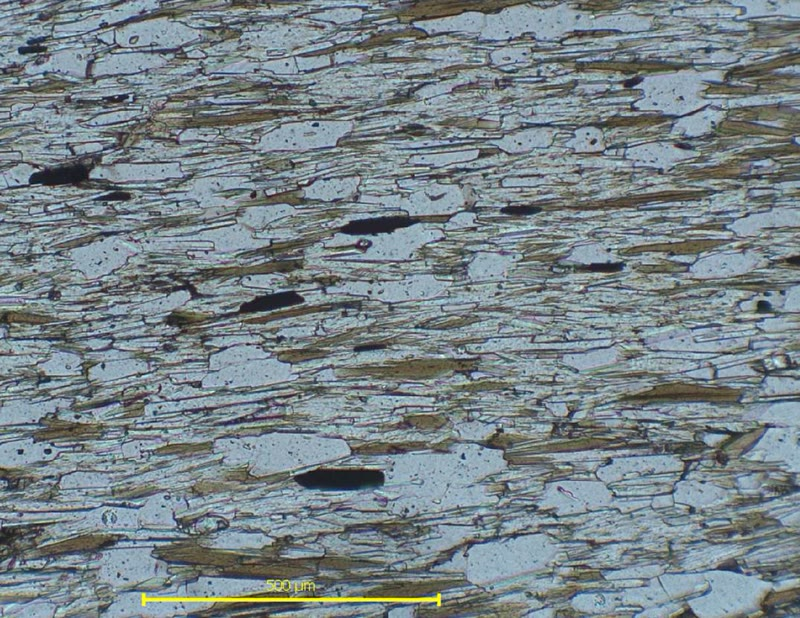
\includegraphics[height=4.3cm]{images/book2/g12-geoloshe-slaty-cleavage.jpg}\hspace{0.03\linewidth}%
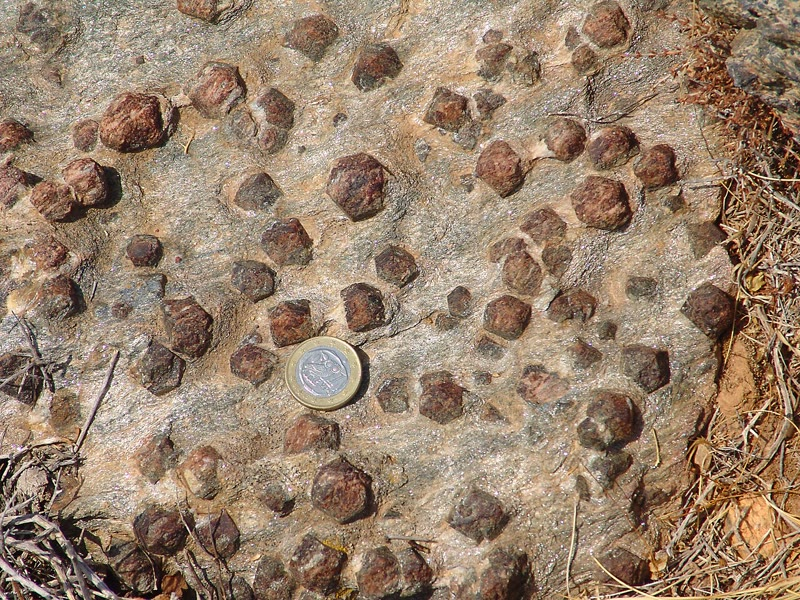
\includegraphics[height=4.3cm]{images/book2/g12-churchard-syros-garnet-schist.jpg}

\smallskip
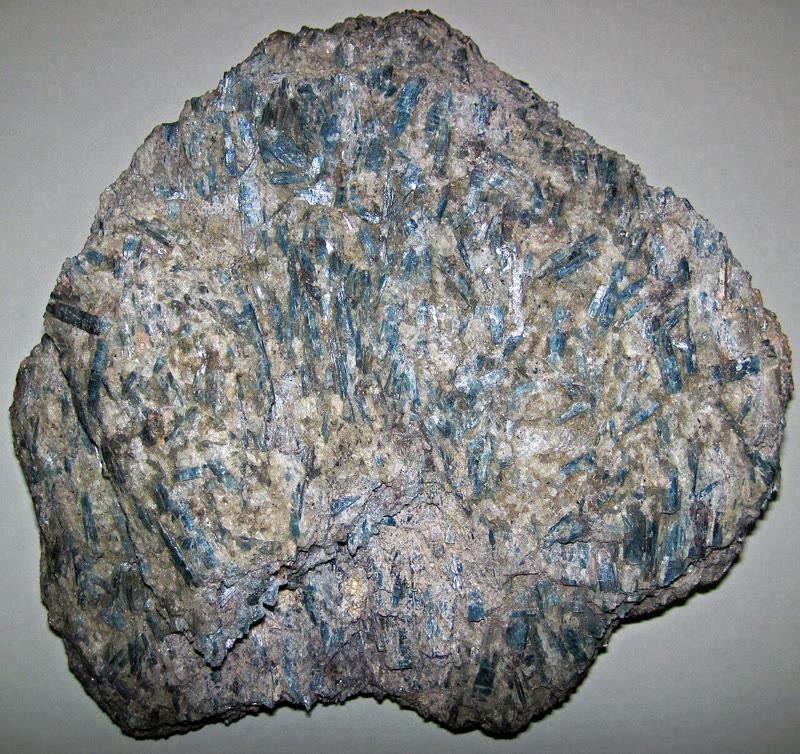
\includegraphics[height=4.3cm]{images/book2/g12-stjohn-kyanite-schist.jpg}\hspace{0.03\linewidth}%
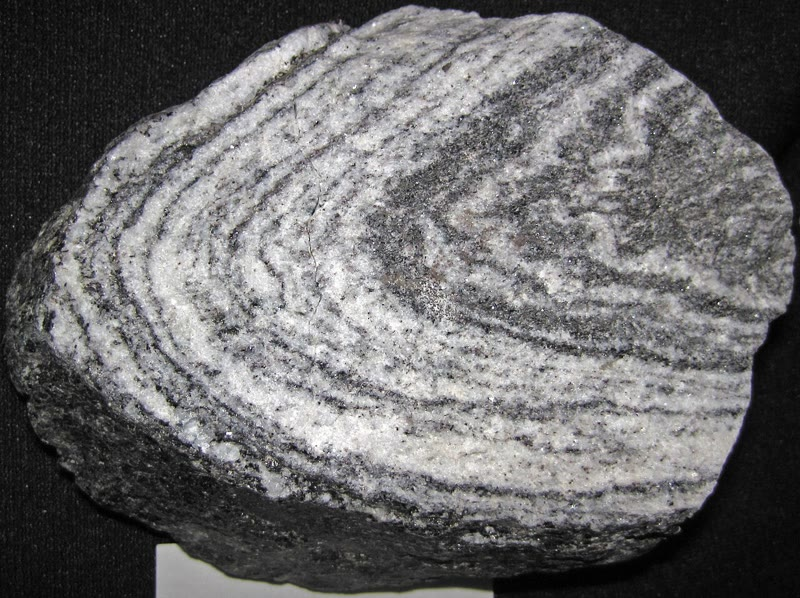
\includegraphics[height=4.3cm]{images/book2/g12-stjohn-gneiss.jpg}

{\small Linksboven: een leisteen onder de microscoop (het gele streepje is
\qty{500}{\micro\metre}): zijn micaschilfers liggen allemaal dezelfde kant op.
Rechtsboven: een granaat-micaschist op het eiland Syros; de munt is
\qty{23}{mm} breed. Linksonder: een schist met blauwe lamellen kyaniet.
Rechtsonder: een gneis met banden kwarts (licht) en biotiet
(donker). Foto's Geoloshe (CC0), Graeme Churchard (CC~BY~2.0) en James
St.~John (CC~BY~2.0).}
\end{omfigure}
% ledger: photo:g12-slaty-cleavage, photo:g12-syros-schist, photo:g12-kyanite-schist, photo:g12-gneiss

Langs een gewone \omterm{def:g11:lithosphere-asthenosphere:geotherm}{geotherm} ontstaat leisteen tussen ongeveer 5 en \qty{10}{km}
diepte, fylliet tussen 10 en 15, schist tussen 15 en 20, en gneis tussen
20 en \qty{25}{km}; nog dieper begint het gesteente hier en daar te smelten. De
\omterm{def:g12:metamorphic-rocks:foliation}{foliatie} legt de richting van de samendrukking vast: ze ontstaat dwars op de
\omterm{def:g12:mountain-building:shortening}{verkorting} die gebergten bouwt (\cref{ch:g12:mountain-building}), en de
oorspronkelijke gelaagdheid van de modder is soms nog te zien terwijl ze haar onder een hoek kruist.
% ledger: earle:settings, earle:foliation

Gesteenten zonder platte of langwerpige mineralen tonen geen \omterm{def:g12:metamorphic-rocks:foliation}{foliatie}, zelfs niet wanneer ze
worden samengeperst. Een kalksteen wordt een \textbf{marmer}, uit grotere kristallen
calciet waarin de fossielen zijn uitgewist; een zandsteen wordt een
\textbf{kwartsiet}, waarvan de kwartskorrels in elkaar zijn gegroeid; en een
modder die wordt verhit zonder te worden samengeperst, wordt een hard, fijnkorrelig gesteente zonder
\omterm{def:g12:metamorphic-rocks:foliation}{foliatie}, een \textbf{hoornfels}.
% ledger: earle:foliation, earle:contact

\section{Contact- en regionale metamorfose}

\begin{definition}[Contactmetamorfose; regionale metamorfose; aureool]\label{def:g12:metamorphic-rocks:contact-regional}
\emph{Contactmetamorfose}\index{contactmetamorfose} is de \omterm{def:g12:metamorphic-rocks:metamorphism}{metamorfose}
van gesteenten die zijn verhit door een magmalichaam dat erin is binnengedrongen; ze blijft beperkt tot
een zone rond de \omterm{def:g11:igneous-rocks:intrusion}{intrusie}, haar \emph{aureool}\index{aureool}, waarin de
graad naar het contact toe stijgt. \emph{Regionale
metamorfose}\index{regionale metamorfose} treft gesteenten die diep zijn begraven over
grote gebieden, meestal waar platen convergeren; de gesteenten worden zowel samengeperst als
verhit, en zijn bijna altijd gefolieerd.
\end{definition}
% ledger: earle:contact, earle:regional, tulane:metamorphism

\subsection{Rond een magmalichaam}

Een magmalichaam van ongeveer \qty{1000}{\celsius} dat in de koude bovenkorst
opstijgt, verhit de gesteenten eromheen. Hun temperatuur kan 300 tot meer
dan \qty{800}{\celsius} bereiken, bij de lage drukken van geringe diepten. De
\omterm{def:g12:metamorphic-rocks:contact-regional}{aureool} is smal: een paar centimeter rond een dunne magmaplaat, tot
enkele tientallen meter rond een groot lichaam. Zijn gesteenten worden verhit zonder
te worden samengeperst, dus zijn ze niet gefolieerd: modder wordt hoornfels, kalksteen
marmer, zandsteen kwartsiet. Een magmalichaam dat zich diep vestigt in gesteenten die
al heet zijn, maakt nauwelijks een \omterm{def:g12:metamorphic-rocks:contact-regional}{aureool}.
% ledger: earle:contact, earle:settings (magma bodies around 1000 degC)

\begin{omfigure}
\begin{tikzpicture}[font=\scriptsize]
  \def\pluton{(3.0,0) .. controls (3.0,2.3) and (7.0,2.3) .. (7.0,0) -- cycle}
  \def\aureole{(2.45,0) .. controls (2.45,2.95) and (7.55,2.95) .. (7.55,0) -- cycle}
  \fill[lith sandstone] (0,0) rectangle (10,0.8);
  \fill[lith limestone] (0,0.8) rectangle (10,1.6);
  \fill[lith shale] (0,1.6) rectangle (10,3);
  \fill[omThm, opacity=0.30] \aureole;
  \draw[omThm, line width=0.6pt, dashed] (2.45,0) .. controls (2.45,2.95) and (7.55,2.95) .. (7.55,0);
  \fill[lith granite] \pluton;
  \draw[black!70, line width=0.6pt] (3.0,0) .. controls (3.0,2.3) and (7.0,2.3) .. (7.0,0);
  \draw[black!60] (0,0) rectangle (10,3);
  \node[fill=white, inner sep=1.5pt] at (5,0.45) {graniet (ooit magma)};
  \draw[black!70] (6.0,1.95) -- (10.6,2.4) node[right] {hoornfels, uit modder};
  \draw[black!70] (7.0,1.2) -- (10.6,1.2) node[right] {marmer, uit kalksteen};
  \draw[black!70] (7.25,0.4) -- (10.6,0.4) node[right] {kwartsiet, uit zandsteen};
  \node[left] at (0,2.3) {schalie};
  \node[left] at (0,1.2) {kalksteen};
  \node[left] at (0,0.4) {zandsteen};
  \draw[omThm] (4.2,2.05) -- (3.4,3.25) node[above, omThm] {aureool};
\end{tikzpicture}

{\small \omterm{def:g12:metamorphic-rocks:contact-regional}{Contactmetamorfose}, in doorsnede: een magmalichaam is opgestegen
in gelaagde sedimentaire gesteenten en heeft er een smalle \omterm{def:g12:metamorphic-rocks:contact-regional}{aureool} (rood) omheen verhit,
waarvan de gesteenten herkristalliseren zonder te worden samengeperst. Schematisch: echte aureolen
zijn centimeters tot tientallen meters breed.}
\end{omfigure}
% ledger: earle:contact

\subsection{Onder een gebergtegordel}

\omterm{def:g12:metamorphic-rocks:contact-regional}{Regionale metamorfose} vraagt begraving tot 10 of \qty{20}{km}, dus treft ze
duizenden vierkante kilometers tegelijk. De waarschijnlijkste plaats is de \omterm{def:g12:continental-crust:root}{wortel} van een
gebergtegordel, waar botsing de korst verdikt en haar gesteenten omlaag duwt
(\cref{ch:g12:mountain-building}). In een oude gordel waarvan de zones in kaart zijn
gebracht, werden de gesteenten van de sillimanietzone verhit tot boven
\qty{700}{\celsius} en 20 tot \qty{25}{km} diep begraven, terwijl die van de
buitenste chlorietzone waarschijnlijk nooit dieper dan ongeveer \qty{5}{km} werden begraven.
De bergen erboven werden daarna over tientallen miljoenen jaren afgesleten; terwijl
de last werd weggenomen, steeg de dikke korst weer op, en de eens diepe zones
liggen nu aan het oppervlak (\cref{ch:g12:destruction-of-mountains}).
% ledger: earle:regional

\subsection{Drie geothermen}

De \omterm{def:g12:metamorphic-rocks:polymorph}{polymorfen} tonen in één oogopslag dat dezelfde diepte niet overal hetzelfde
gesteente betekent: dat hangt af van de \omterm{def:g11:lithosphere-asthenosphere:geotherm}{geotherm}. De figuur van de \omterm{def:g12:metamorphic-rocks:polymorph}{polymorfen}
draagt er drie.
% ledger: earle:settings

\begin{itemize}
  \item Een \textbf{gewone} \omterm{def:g11:lithosphere-asthenosphere:geotherm}{geotherm}, ongeveer \qty{30}{\celsius} per
        kilometer: de temperatuur bereikt ongeveer \qty{300}{\celsius} op
        \qty{10}{km}. Hij loopt onder het tripelpunt door, dus maakt kyaniet
        meteen plaats voor sillimaniet, bij ongeveer \qty{574}{\celsius} en
        \qty{18.8}{km}.
  \item Een \omterm{def:g11:lithosphere-asthenosphere:geotherm}{geotherm} van een \textbf{vulkanisch gebied}, 40 tot \qty{50}{\celsius} per
        kilometer, steiler gemaakt door de warmte van opstijgend magma: de gesteenten bereiken
        hoge temperaturen op geringe diepten. Bij \qty{50}{\celsius} per
        kilometer verschijnt andalusiet op ongeveer \qty{6.6}{km} en maakt het plaats voor
        sillimaniet op ongeveer \qty{10.9}{km}, \qty{553}{\celsius}.
  \item De \omterm{def:g11:lithosphere-asthenosphere:geotherm}{geotherm} van een \textbf{\omterm{def:g11:subduction-zones:subduction}{subductiezone}}, onder
        \qty{10}{\celsius} per kilometer: de \omterm{def:g11:ocean-ridges:oceanic-lithosphere}{oceanische korst} die omlaag wordt gevoerd,
        blijft enkele honderden graden kouder dan de mantel eromheen. Op
        \qty{36}{km} is ze maar ongeveer \qty{370}{\celsius}, diep in het
        kyanietveld. Dit is het koude hogedrukpad waarop basalt
        \omterm{def:g11:subduction-zones:eclogite}{blauwschist} wordt en daarna \omterm{def:g11:subduction-zones:eclogite}{eclogiet}, op ongeveer \qty{35}{km}.
\end{itemize}
% values: cross_30_0 573.6 degC 18.79 km; cross_50_0 340.1 degC 6.60 km; cross_50_1 553.0 degC 10.86 km; sub10_T_at_1gpa 370.2 (al2sio5.py)
% ledger: earle:settings

Zo draagt elk metamorf gesteente een verslag van de \omterm{def:g11:lithosphere-asthenosphere:geotherm}{geotherm} waaronder het
is ontstaan, en van de plaattektonische setting erachter: andalusiet en hoornfels wijzen op
warmte op geringe diepten, rond magmalichamen; kyaniet- en sillimanietschisten
en gneisen op de diepe \omterm{def:g12:continental-crust:root}{wortels} van gebergtegordels; \omterm{def:g11:subduction-zones:eclogite}{blauwschisten} en
\omterm{def:g11:subduction-zones:eclogite}{eclogieten} op \omterm{def:g11:subduction-zones:subduction}{subductiezones}. De meeste van deze gesteenten konden alleen worden gezien
omdat ze naar het oppervlak terugkwamen zonder terug te veranderen. Terwijl ze opstijgen
en afkoelen, vertragen hun reacties, en het water dat de omgekeerde
reacties nodig zouden hebben, is op de weg naar beneden ontsnapt.
% ledger: earle:settings, earle:contact, tulane:metamorphism (retrograde metamorphism uncommon)

\section{Oefeningen}

\begin{exercise}[$\star$]\label{exo:g12:metamorphic-rocks:1}
Geef het woord: (a) mineralen met dezelfde samenstelling maar verschillende
kristalstructuren; (b) de lijn op een kaart waar een \omterm{def:g12:metamorphic-rocks:index-mineral}{indexmineraal} voor het eerst verschijnt;
(c) de zone van verhitte gesteenten rond een magmalichaam; (d) de evenwijdige vlakken
gevormd door op één lijn liggende platte mineralen; (e) de druk door het gewicht van de
gesteenten erboven.
\end{exercise}

\begin{exercise}[$\star$]\label{exo:g12:metamorphic-rocks:2}
Noem het metamorfe gesteente dat elk \omterm{def:g10:soil-formation:weathering-profile}{moedergesteente} wordt: (1) een kalksteen;
(2) een zandsteen; (3) een modder, bij lage graad onder samendrukking; (4) een modder, bij hoge
graad; (5) een modder, verhit door een magmalichaam zonder te worden samengeperst.
\end{exercise}

\begin{exercise}[$\star$]\label{exo:g12:metamorphic-rocks:3}
Bereken met $\rho = \qty{2830}{kg/m^3}$ en $g = \qty{9.81}{m/s^2}$ de
\omterm{def:g12:metamorphic-rocks:lithostatic}{lithostatische druk}, in \unit{GPa}, op \qty{10}{km} en op \qty{20}{km}.
\end{exercise}

\begin{exercise}[$\star$]\label{exo:g12:metamorphic-rocks:4}
Welk mineraal is op het diagram van de \omterm{def:g12:metamorphic-rocks:polymorph}{polymorfen} van \ce{Al2SiO5} stabiel
(1) bij \qty{400}{\celsius} en \qty{0.6}{GPa}; (2) bij \qty{500}{\celsius}
en \qty{0.2}{GPa}; (3) bij \qty{750}{\celsius} en \qty{0.3}{GPa}?
\end{exercise}

\begin{exercise}[$\star$]\label{exo:g12:metamorphic-rocks:5}
(1) Zet op volgorde van stijgende graad: schist, leisteen, gneis, fylliet. (2) In
welke ervan kun je de mica's met het blote oog zien? (3) Welke toont
lichte en donkere banden?
\end{exercise}

\begin{exercise}[$\star\star$]\label{exo:g12:metamorphic-rocks:6}
(1) Bereken de \omterm{def:g12:metamorphic-rocks:lithostatic}{lithostatische druk} aan de basis van een korst van \qty{35}{km}
dik ($\rho = \qty{2830}{kg/m^3}$) en druk die uit in atmosfeer
($\qty{1}{atm} = \qty{101325}{Pa}$). (2) Bereken de druk op de bodem
van een oceaan van \qty{4}{km} diep, met zeewater van dichtheid
\qty{1025}{kg/m^3}. (3) Hoeveel keer groter is de eerste?
\end{exercise}

\begin{exercise}[$\star\star$]\label{exo:g12:metamorphic-rocks:7}
Het tripelpunt van \ce{Al2SiO5} ligt bij \qty{504}{\celsius} en
\qty{0.375}{GPa}. (1) Op welke diepte wordt die druk bereikt ($\rho =
\qty{2830}{kg/m^3}$)? (2) Welke \omterm{def:g11:lithosphere-asthenosphere:geotherm}{geothermische gradiënt}, vertrekkend van
\qty{10}{\celsius} aan het oppervlak, loopt er precies door? (3) Is een gesteente
dat alle drie de \omterm{def:g12:metamorphic-rocks:polymorph}{polymorfen} bevat, waarschijnlijk algemeen?
\end{exercise}

\begin{exercise}[$\star\star$]\label{exo:g12:metamorphic-rocks:8}
Op de foto van de granaatschist van Syros zijn de grootste granaten
ongeveer een derde zo breed als de munt, die \qty{23}{mm} meet. (1) Schat
hun diameter. (2) Als de diameter van een granaat met ongeveer \qty{1}{mm} per
miljoen jaar groeit, hoe lang deden ze er dan over om te groeien? (3) Wat zegt dat
over de tijd die een gesteente op diepte doorbrengt?
\end{exercise}

\begin{exercise}[$\star\star$]\label{exo:g12:metamorphic-rocks:9}
Een geoloog die \qty{24}{km} westwaarts over een oude gebergtegordel wandelt,
noteert gesteenten die uit modder zijn ontstaan. Aan het begin bevatten ze alleen chloriet en biotiet;
de eerste granaat verschijnt na \qty{6}{km}, de eerste stauroliet na
\qty{11}{km}, de eerste kyaniet na \qty{15}{km}, de eerste sillimaniet
na \qty{20}{km}. (1) Hoeveel isograden werden er overschreden? Noem ze op volgorde.
(2) In welke richting stijgt de graad? (3) Waar werden de gesteenten het diepst
begraven, en hoe heet werden ze daar ruwweg?
\end{exercise}

\begin{exercise}[$\star\star$]\label{exo:g12:metamorphic-rocks:10}
Een magmalichaam stijgt dicht bij het oppervlak op in lagen modder, kalksteen en zandsteen. (1) Noem het gesteente dat elke laag ernaast wordt. (2) Waarom zijn deze
gesteenten niet gefolieerd? (3) Een tweede magmalichaam vestigt zich op \qty{20}{km} diepte, in
gesteenten die al bijna \qty{500}{\celsius} zijn. Waarom maakt het nauwelijks een \omterm{def:g12:metamorphic-rocks:contact-regional}{aureool}?
\end{exercise}

\begin{exercise}[$\star\star$]\label{exo:g12:metamorphic-rocks:11}
Een laag modder wordt tijdens een botsing vanuit het oosten en het westen samengeperst,
en laat mica's groeien terwijl ze wordt verhit. (1) Hoe liggen de mica's: met hun platte vlakken
naar oost--west of naar noord--zuid gericht? (2) Is de \omterm{def:g12:metamorphic-rocks:foliation}{foliatie} die ontstaat
horizontaal of verticaal? (3) Een marmer en een kwartsiet die op dezelfde
manier zijn samengeperst, tonen geen \omterm{def:g12:metamorphic-rocks:foliation}{foliatie}. Waarom?
\end{exercise}

\begin{exercise}[$\star\star\star$]\label{exo:g12:metamorphic-rocks:12}
Tussen 500 en \qty{700}{\celsius} ligt de grens tussen kyaniet en sillimaniet
dicht bij de rechte $P = 0.577 + 0.00209\,(T - 600)$, met $P$ in
\unit{GPa} en $T$ in \unit{\celsius}. Een gewone \omterm{def:g11:lithosphere-asthenosphere:geotherm}{geotherm} is $T = 10 + 30z$
($z$ in \unit{km}), en $P = 0.0278\,z$. (1) Schrijf de \omterm{def:g11:lithosphere-asthenosphere:geotherm}{geotherm} als $P$ als
functie van $T$. (2) Bepaal waar hij de grens snijdt: temperatuur, druk,
diepte. (3) Welke \omterm{def:g12:metamorphic-rocks:polymorph}{polymorf} is langs deze \omterm{def:g11:lithosphere-asthenosphere:geotherm}{geotherm} stabiel net boven die
diepte, en welke net eronder?
\end{exercise}

\begin{exercise}[$\star\star\star$]\label{exo:g12:metamorphic-rocks:13}
(1) Wat is langs een subductiegeotherm van \qty{10}{\celsius} per kilometer, vertrekkend
van \qty{10}{\celsius}, de temperatuur op \qty{35}{km}, waar
\omterm{def:g11:subduction-zones:eclogite}{eclogiet} ontstaat? (2) Wat is ze langs een gewone \omterm{def:g11:lithosphere-asthenosphere:geotherm}{geotherm} van
\qty{30}{\celsius} per kilometer? (3) Zet beide punten uit op het diagram van
de \omterm{def:g12:metamorphic-rocks:polymorph}{polymorfen}: welke \omterm{def:g12:metamorphic-rocks:polymorph}{polymorf} is stabiel in het eerste? (4) Waarom ontstaan
\omterm{def:g11:subduction-zones:eclogite}{blauwschisten} en \omterm{def:g11:subduction-zones:eclogite}{eclogieten} in \omterm{def:g11:subduction-zones:subduction}{subductiezones} en bijna nergens anders?
\end{exercise}

\begin{exercise}[$\star\star\star$]\label{exo:g12:metamorphic-rocks:14}
De dichtheden van kyaniet, sillimaniet en andalusiet zijn \num{3.61},
\num{3.24} en \qty{3.15}{g/cm^3}. (1) Bereken het volume van \qty{1}{kg} van
elk, in \unit{cm^3}. (2) Met welk percentage is kyaniet kleiner dan
andalusiet met dezelfde massa? (3) Leg uit, met het idee dat een hoge druk
de rangschikking begunstigt die de minste ruimte inneemt, waarom kyaniet het
hogedrukveld van het diagram bezet.
\end{exercise}

\begin{exercise}[$\star\star\star$]\label{exo:g12:metamorphic-rocks:15}
In een oude gebergtegordel werden de gesteenten van de sillimanietzone verhit tot boven
\qty{700}{\celsius} en 20 tot \qty{25}{km} diep begraven. (1) Bereken de
druk op 20 en op \qty{25}{km}. (2) Bepaal met de rechte van
oefening~12 de laagste temperatuur waarbij sillimaniet stabiel is bij
elk van deze drukken. Is \qty{700}{\celsius} in overeenstemming met sillimaniet?
(3) Welke \omterm{def:g11:lithosphere-asthenosphere:geotherm}{geothermische gradiënten}, vanaf \qty{10}{\celsius} aan het oppervlak, volgen uit
\qty{700}{\celsius} op 20 en op \qty{25}{km}? (4) De gesteenten kwamen
ongeveer 40 miljoen jaar later aan het oppervlak. Met welke gemiddelde snelheid werd
het gesteente erboven weggehaald, in \unit{mm} per jaar?
\end{exercise}

\begin{problem}[{Weekendprobleem --- de geschiedenis van een kyanietschist}]
\label{pb:g12:metamorphic-rocks:1}
% ledger: hm93:table11, cm95:crust, earle:controls, earle:settings, earle:regional, tulane:roots, tulane:metamorphism, iugs:barrow; Book 3: webmineral:polymorphs; Book 1: ussa76:sea-level
% values: pb_z_km 25.214, pb_grad 23.4, pb_kysil_P_at_600_gpa 0.577 (al2sio5.py); t_on_kysil(7.0) = 658.9
Een schist die in de kern van een oude gebergtegordel is verzameld, bevat muscoviet,
biotiet, kwarts, granaten tot \qty{8}{mm} breed, en blauwe lamellen
kyaniet; hij bevat geen sillimaniet en geen andalusiet. Laboratoriumanalyses van
zijn granaat en biotiet geven de omstandigheden waaronder hij kristalliseerde:
ongeveer \qty{600}{\celsius} en \qty{0.70}{GPa}. Neem $\rho =
\qty{2830}{kg/m^3}$, $g = \qty{9.81}{m/s^2}$, \qty{10}{\celsius} aan het
oppervlak, en de grenslijn tussen kyaniet en sillimaniet van oefening~12, $P = 0.577 +
0.00209\,(T - 600)$.

\medskip
\noindent\textbf{Deel I --- De mineralen.}
\begin{enumerate}
  \item Waarom heet het gesteente een schist? Welke van zijn mineralen vormen de
        \omterm{def:g12:metamorphic-rocks:foliation}{schistositeit}?
  \item Kyaniet, andalusiet en sillimaniet delen één formule. Schrijf die op, en
        geef het woord voor zulke mineralen.
  \item De dichtheden van kyaniet en andalusiet zijn \num{3.61} en
        \qty{3.15}{g/cm^3}. Met welk percentage is het volume van een kilogram
        kyaniet kleiner? Welke wordt door druk begunstigd?
  \item Tot welke zone behoort het gesteente in de reeks indexmineralen van gesteenten uit modder? Welke isograden overschreed het op zijn weg naar beneden?
  \item Als de diameter van de granaten met ongeveer \qty{1}{mm} per miljoen
        jaar groeide, hoe lang deden de grootste erover om te groeien?
\end{enumerate}

\medskip
\noindent\textbf{Deel II --- Druk en temperatuur.}
\begin{enumerate}[resume]
  \item Boven welke druk is kyaniet bij \qty{600}{\celsius} stabiel in plaats
        van sillimaniet?
  \item Controleer dat het punt (\qty{600}{\celsius}, \qty{0.70}{GPa}) in
        het kyanietveld ligt.
  \item Het ontbrekende sillimaniet geeft een laagste druk bij
        \qty{600}{\celsius}. Welke is dat?
  \item Als het gesteente bij \qty{0.70}{GPa} verder was verhit, bij welke
        temperatuur zou zijn kyaniet dan sillimaniet zijn geworden?
  \item Druk \qty{0.70}{GPa} uit in kilobar ($\qty{1}{kbar} =
        \qty{e8}{Pa}$) en in atmosfeer ($\qty{1}{atm} = \qty{101325}{Pa}$).
\end{enumerate}

\medskip
\noindent\textbf{Deel III --- De begravingsdiepte.}
\begin{enumerate}[resume]
  \item Met hoeveel megapascal stijgt de \omterm{def:g12:metamorphic-rocks:lithostatic}{lithostatische druk} per
        kilometer?
  \item Op welke diepte lag de schist toen hij kristalliseerde?
  \item Wat is de kleinste diepte die het ontbrekende sillimaniet toelaat
        (vraag 8)?
  \item Doe vraag 12 opnieuw met een dichtheid van \qty{2700}{kg/m^3} voor de gesteenten
        erboven. Met welk percentage verandert de diepte?
  \item Een \omterm{def:g12:continental-crust:continental-crust}{continentale korst} is gewoonlijk 35 tot \qty{40}{km} dik, en 50 tot
        \qty{70}{km} onder gebergtegordels. Kristalliseerde de schist in de
        korst of in de mantel?
\end{enumerate}

\medskip
\noindent\textbf{Deel IV --- De geotherm, en de weg terug naar boven.}
\begin{enumerate}[resume]
  \item Welke gemiddelde \omterm{def:g11:lithosphere-asthenosphere:geotherm}{geothermische gradiënt} volgt uit \qty{600}{\celsius} op die diepte?
  \item Vergelijk die met de gradiënten van een \omterm{def:g11:subduction-zones:subduction}{subductiezone}, een gewone
        korst en een vulkanisch gebied. Welke soort \omterm{def:g12:metamorphic-rocks:metamorphism}{metamorfose} maakte het gesteente?
  \item Wat zou langs een gewone \omterm{def:g11:lithosphere-asthenosphere:geotherm}{geotherm} van \qty{30}{\celsius} per kilometer de
        temperatuur zijn op de diepte van vraag 12? Welke
        \omterm{def:g12:metamorphic-rocks:polymorph}{polymorf} zou dan bij \qty{0.70}{GPa} stabiel zijn?
  \item Om de schist naar het oppervlak te brengen, moest al het gesteente erboven worden
        weggehaald. Hoe lang duurde dat bij een gemiddelde snelheid van \qty{0.5}{mm} per jaar?
  \item Waarom werd het kyaniet op de weg naar boven niet weer andalusiet?
  \item Vat samen: op welke diepte kristalliseerde deze kyanietschist?
\end{enumerate}
\end{problem}
